%\documentclass[aspectratio=169]{beamer}
\documentclass[aspectratio=169,handout]{beamer}
\usetheme{metropolis}
\usepackage{times}
\usepackage{tikz}
\usetikzlibrary{patterns}
\tikzset{>=latex} % for LaTeX arrow head
\usepackage{calc} % for simple arithmetic
\usepackage{amsmath}
\usepackage{verbatim}
\usepackage{adjustbox}
\usepackage{listings}
\usepackage{verbatim}
\usepackage{array}
\usetikzlibrary{arrows,automata}
\setbeamercolor{progress bar}{fg=red,bg=}
\lstset{language=C,
  basicstyle=\ttfamily,
  keywordstyle=\color{blue}\ttfamily,
  stringstyle=\color{gray}\ttfamily,
  commentstyle=\color{green}\ttfamily,
  morecomment=[l][\color{blue}]{\#}
}

\title{Der Cyber-Bankraub von Bangladesch}
\date{FrOSCon --- 22. August 2021}
\author{Lars A. Wallenborn}
\institute{Mit Malware Analyse Großkriminellen auf die Spur kommen}
\begin{document}
\tikzstyle{every picture}+=[remember picture]

\maketitle
\section{Intro}
\begin{frame}{whoami}
  Lars A. Wallenborn\\
  lars@wallenborn.net\\
  @larsborn\\
  \vspace{1cm}
  Seit 2004 Freiberufler im IT Bereich\\
  2013 Diplom in Mathematik @ Uni Bonn\\
  2014 - 2015 Softwareentwickler @ Bonn\\
  Seit 2015: Security Researcher @ CrowdStrike\\
  Seit 2021: Podcaster @ https://armchairinvestigators.de/
\end{frame}

\begin{frame}{Agenda}
  \begin{enumerate}
    \item Was ist passiert?
    \item Reverse Engineering
      \begin{enumerate}
        \item Was ist das?
        \item Assembly
        \item Tools
        \item Ghidra
      \end{enumerate}
    \item Demo!
  \end{enumerate}
\end{frame}

\newcommand{\fullslide}[3]{\begin{frame}[plain]
  \begin{tikzpicture}[remember picture,overlay]
  \node[at=(current page.center)]{
    \includegraphics[width=\paperwidth]{images/#1}
    };
    \pgfsetfillopacity{0.7}
    \node[at=(current page.center)]{
      \begin{beamercolorbox}[sep=0.5cm,wd=.7\paperwidth]{title}%
        \centering
        \pgfsetfillopacity{1}%
        \LARGE
        #3
      \end{beamercolorbox}
    };
    \node[anchor=south east, at=(current page.south east), text=white]{\pgfsetfillopacity{0.8}\tiny Quelle: #2};
  \end{tikzpicture}
\end{frame}}

\section{Was ist passiert?}


\fullslide{printer.jpg}{https://unsplash.com/photos/bat9Y6pSoTI}{\begin{itemize}
    \pause
  \item Drucker ausgefallen\pause
  \item 5./6. Februar 2016\pause
\item Zentralbank von Bangladesch
\end{itemize}}

\fullslide{bangladesh.jpg}{https://unsplash.com/photos/qIUb3VNmxjI}{\begin{itemize}
\pause
\item Entwicklungsland östlich von Indien\pause
\item 165 Millionen Einwohnern\pause
\item 220 Milliarden USD BIP
\end{itemize}}

\fullslide{bangladesh-bank-building.jpg}{https://commons.wikimedia.org/wiki/File:Bangladesh\_Bank\_(33398162476).jpg}{\begin{itemize}
\pause
\item Bangladesh Bank\pause
\item Zentralbank des Landes\pause
\item Notenbank für die Stabilität des Taka
\end{itemize}}

\fullslide{network.jpg}{https://unsplash.com/photos/rhNff6hB41s}{\begin{itemize}
\item Donnerstag, 4. Februar 2016\pause
\item Feierabend\pause
\item 35 SWIFT Nachrichten gehen an NYFed\pause
\item Eine Milliarde Dollar
\end{itemize}}

\fullslide{nyfed.jpg}{https://en.wikipedia.org/wiki/File:2015\_Federal\_Reserve\_Bank\_of\_New\_York\_from\_west.jpg}{\begin{itemize}
\item Freitag, 5. Februar 2016\pause
\item NYFed versucht Bangladesh Bank zu kontaktieren\pause
\item Freitag (Muslims) $\approx$ Sonntag (Christen)
\end{itemize}}

\fullslide{hours-later.jpg}{https://unsplash.com/photos/Ox-x45IaxSA}{\begin{itemize}
\item Samstag, 6. Februar 2016
\end{itemize}}

\fullslide{panic.jpg}{https://unsplash.com/photos/7vXXYBzNO-U}{\begin{itemize}
\item Sonntag, 7. Februar 2016\pause
\item SWIFT Transaktion soll abgebrochen werden (MT 192?)\pause
\item NYFed hat natürlich Sonntag
\end{itemize}}

\fullslide{rcbc.jpg}{https://commons.wikimedia.org/wiki/File:466Ayala\_Alabang\_Muntinlupa\_Las\_Pi\%C3\%B1as\_City\_39.jpg}{\begin{itemize}
\item Montag, 8. Februar 2016\pause
\item NYFed leitet die Anfrage weiter\pause
\item insb. an RCBC Bank auf den Philippinen\pause
\item Dort wird aber gerade ein (chinesischer) Feiertag gefeiert
\end{itemize}}

\fullslide{money.jpg}{https://unsplash.com/photos/IFSvUMApzsI}{\begin{itemize}
\item Dienstag, 9. Februar 2016\pause
\item 58 Millionen USD sind bereits abgehoben\pause
\item Werden über Spielcasinos gewaschen und verschwinden nach China
\end{itemize}}

\begin{frame}{Zeitlicher Verlauf}
  \makebox[\textwidth][c]{\scalebox{1.8}{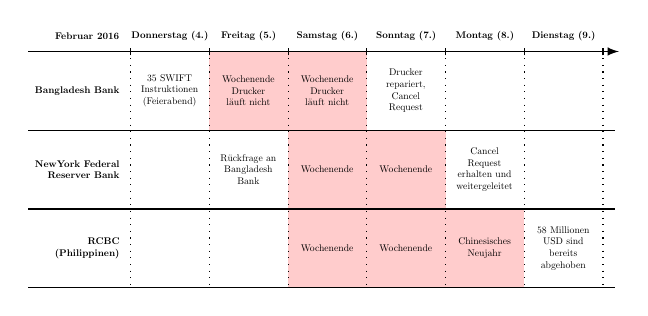
\begin{tikzpicture}[every node/.style={scale=0.35}]
  % red fills
  \uncover<3->{
    \fill[red!20!white] (1.5,0) rectangle (3.5,-1);
    \fill[red!20!white] (2.5,-1) rectangle (4.5,-2);
    \fill[red!20!white] (2.5,-2) rectangle (5.5,-3);
  }
  % Zeitachse
  \draw[->] (-0.8, 0) -- (6.7, 0);

  % horizontale Striche
  \foreach \x in {1,...,3}
    \draw (-0.8, -\x) -- (6.65, -\x);

    % Achsenmarkierungen
  \foreach \x in {0,...,6}
    \draw (\x+0.5, -0.05) -- (\x+0.5,0.05);

  % Titel
  \draw (0.4, 0.2) node[font=\bfseries,left]{Februar 2016};
  \foreach \c [count=\x from 1] in {{Donnerstag (4.)}, {Freitag (5.)}, {Samstag (6.)}, {Sonntag (7.)}, {Montag (8.)}, {Dienstag (9.)}}
    \draw (\x, 0.2) node[font=\bfseries]{\c};

  % Striche nach unten
  \foreach \x in {0,...,6}
  \draw[dotted] (\x+0.5, 0) -- (\x+0.5, -3);

  % Linke Spalte
  \uncover<2->{
    \foreach \c [count=\x from 0] in {{Bangladesh Bank},{NewYork Federal Reserver Bank}, {RCBC\\(Philippinen)}}
      \draw (-0.2, -\x-0.5) node[text width=3.2cm,align=right,font=\bfseries]{\c};
  }
  % erste Zeile
  \uncover<4->{
    \foreach \c [count=\x from 1] in {{35 SWIFT Instruktionen (Feierabend)}, {Wochenende\\Drucker läuft nicht}, {Wochenende\\Drucker läuft nicht}, {Drucker repariert, Cancel Request}}
      \draw (\x-0.45, -0.5) node[right,text width=2.3cm,align=center]{\c};
  }

  % zweite Zeile
  \uncover<5->{
    \foreach \c [count=\x from 2] in {{Rückfrage an Bangladesh Bank}, {Wochenende}, {Wochenende}, {Cancel Request erhalten und weitergeleitet}}
      \draw (\x-0.45, -1.5) node[right,text width=2.3cm,align=center]{\c};
  }

  % dritte Zeile
  \uncover<6->{
    \foreach \c [count=\x from 3] in {{Wochenende}, {Wochenende}, {Chinesisches Neujahr}, {58 Millionen USD sind bereits abgehoben}}
      \draw (\x-0.45, -2.5) node[right,text width=2.3cm,align=center]{\c};
  }

  \end{tikzpicture}}}
\end{frame}

\fullslide{correction.jpg}{https://unsplash.com/photos/h7-V2KkCECI}{\begin{itemize}
  \pause
  \item nur 4 (von 35) Transaktionen durchgegangen\pause
  \item Heuristiken\pause
  \item "Jupiter Street" vs. "Jupiter Sea Ways"\pause
  \item "fandation"
\end{itemize}}

\fullslide{cool-story.jpg}{https://unsplash.com/photos/WCOCEq81wmc}{\begin{center}
Cool Story Bro
\end{center}}

\section{Was ist Reverse Engineering?}
\begin{frame}{Was ist Reverse Engineering?}
  \begin{itemize}
    \item zu Deutsch: Rückwärtsanalyse\pause
    \item kurz: \emph{RE} oder \emph{reversing}\pause
    \item sehr allgemeiner Ausdruck: \pause einen Produktionsprozess rückwärts durchführen\pause
    \item mit dem Ziel das Design, die Architekture oder --- ganz allgemein --- Wissen über das RE Ziel zu ermitteln
  \end{itemize}
  \pause
  \begin{alertblock}{In diesem Vortrag}\pause
    Konzentrieren wir uns auf:\\
    \begin{center}
      \emph{Reversing von kompilierter Software}
    \end{center}
  \end{alertblock}
\end{frame}

\begin{frame}{Binary Software Reverse Engineering}
  \begin{adjustbox}{max totalsize={.9\textwidth}{.7\textheight},center}
    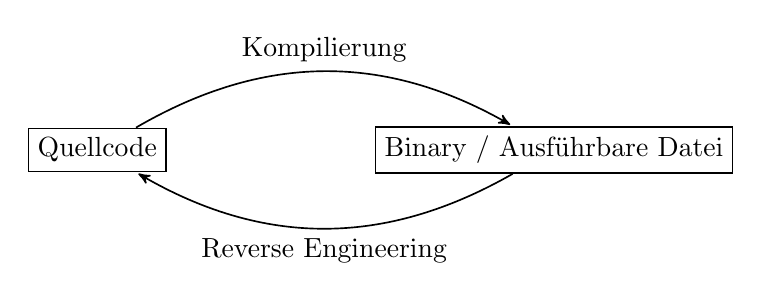
\begin{tikzpicture}[->,>=stealth',shorten >=1pt,auto,node distance=5.8cm,
      semithick]
    \node[rectangle,draw] (A)              {Quellcode};
    \node[rectangle,draw] (B) [right of=A] {Binary / Ausführbare Datei};

    \path (A) edge[bend left] node {Kompilierung} (B);
    \pause
    \path (B) edge[bend left] node {Reverse Engineering} (A);
    \end{tikzpicture}
  \end{adjustbox}
\end{frame}

\section{Assembly}
\begin{frame}[fragile]{Assembly}\pause
  \begin{itemize}
    \item Schwer zu lesende Programmiersprache, die direkt von einer CPU ausgeführt werden kann.\pause
    \item Erlaubt nur sehr einfach Dinge wie addieren oder Speicherzugriffe.\pause
    \item Wird oft im "disassembled" Zustand angezeigt\pause: Anstelle von
    \begin{verbatim}
      90907504
    \end{verbatim}
    \pause schreibt man
    \begin{lstlisting}
      NOP
      NOP
      JNZ 6
    \end{lstlisting}\pause
    \item Sehr zeitaufwendig zu lesen
  \end{itemize}
\end{frame}

\section{Reversing Tools}
\begin{frame}{Reversing Tools}\pause
  \begin{itemize}
    \item IDA \pause (Interactive Disassembler) \pause + HexRays Decompiler\pause
    \item Binary Ninja\pause
    \item RetDec \pause (retargetable decompiler)\pause
    \item Ghidra
  \end{itemize}
\end{frame}

\section{Ghidra}
\begin{frame}{Was ist Ghidra?}
  \begin{itemize}
    \item Existenz ist bekannt seit den Vault7 leaks 2017.\pause
    \item Die NSA kündigte 2019 auf der RSA Konferenz an, dass sie Ghidra als OSS veröffentlichen werden.\pause
    \item Das ist dann auch passiert: https://github.com/NationalSecurityAgency/ghidra\pause
    \item In Java geschriebene GUI.\pause
    \item In C geschriebenes Decompiler backend.\pause
    \item Kann native PE Dateien (.exe-Dateien) \emph{dekompilieren}\pause
    \item (und auch viele andere Formate)
  \end{itemize}
\end{frame}

\begin{frame}{Demo}
  \begin{center}
    \includegraphics[width=0.6\paperwidth]{images/ticket.jpg}
  \end{center}
\end{frame}

\begin{frame}{Danke für die Aufmerksamkeit}
  \begin{itemize}
    \item Angriffe hinterlassen Spuren
    \item Reversing kann man lernen
    \item Mit Reversing kann man solche Spuren analysieren
  \end{itemize}
  Lars A. Wallenborn\\
  lars@wallenborn.net\\
  @larsborn\\
  \vspace{1cm}
  \emph{Eigenwerbung:}\\
  \begin{itemize}
  \item Ich gebe Schulungen im Reverse Engineering: \textbf{mal.re} (mit Jesko Hüttenhain)
    \item Hört in den Podcast rein: \textbf{armchairinvestigators.de} (mit Christian Dietrich)
  \end{itemize}
\end{frame}

\end{document}
